\hsectionENDE{Conceptual Modeling}{Konzeptuelle Modellierung}%
%
%
\begin{questionENDE}{Basics}{Grundlagen}%
\qENDE{%
What is an \emph{entity} and what is an \emph{entity type} in the conceptual modeling stage? %
What is the difference between them? %
What real-world things do they represent?%
}{%
Was ist eine \emph{Entität} und was ist ein \emph{Entitätstyp} in der konzeptuellen Modellierung? %
Was ist der Unterschied zwischen ihnen? %
Welche Dinge der realen Welt repräsentieren sie?%
}%
\end{questionENDE}%
%
\begin{questionENDE}{Basics}{Grundlagen}%
\qENDE{%
What are \emph{attributes} in the conceptual modeling stage? %
What real-world concepts do they represent?%
}{%
Was sind \emph{Attribute} in der konzeptuellen Modellierung? %
Welche Konzepte aus der realen Wert repräsentieren sie?%
}%
\end{questionENDE}%
%
\begin{questionENDE}{Keys}{Schlüssel}%
\qENDE{%
What are \emph{keys} in the conceptual model?%
}{%
Was sind \emph{Schlüssel} im konzeptuellen Modell?%
}%
\end{questionENDE}%
%
\begin{questionENDE}{Keys}{Schlüssel}%
\qENDE{%
What are \emph{(candidate) keys} and \emph{primary keys} in the conceptual model? %
What is the difference between them?%
}{%
Was sind \emph{Schlüssel(kandidaten)} und \emph{Primärschlüssel} im konzeptuellen Modell? %
Was ist der Unterschied zwischen beiden?%
}%
\end{questionENDE}%
%
\begin{questionENDE}{Entities and Attributes}{Entitäten und Attribute}%
\qENDE{%
List the entities, entity types, and attributes in the following text:\\%
\inQuotes{%
The province Anhui has an area of 140\decSep100~$km^2$ and a population of over 61~million people. %
The city Hefei has a GDP of over 180~billion USD an is one of the science centers of China. %
Hefei has several good universities, including USTC, HFUT, Hefei University, and Anhui University.%
}%
}{%
Geben Sie die Entitäten, Entitätstypen und Attribute aus dem folgenden Text an:\\%
\inQuotes{%
Die Provinz Anhui hat eine Fläche von 140\decSep100~$km^2$ und eine Bevölkerung von über 61~Million Menschen. %
Die Stadt Hefei hat ein Bruttosozialprodukt von über 180~Milliarden USD und ist eines der Wissenschaftszentren von China. %
Hefei hat mehrere gute Universitäten, wie \DEzB\ die USTC, HFUT, die Universität Hefei und die Anhui Universität.%
}%
}%
\end{questionENDE}%
%
\begin{questionENDE}{Relationship Cardinality and Modality}{Beziehungskardinalität und -modalität}%
\qENDE{%
Express the following relationship with Crow's Foot notation:~\inQuotes{%
Every person has at least one address. %
An arbitrary number (including~0) of people can live at an address.%
}%
}{%
Drücken Sie die folgende Beziehung mit der Krähenfußnotation aus:~\inQuotes{%
Jede Person hat mindestens eine Adresse. %
Eine beliebige Anzahl (auch~0) Leute können unter einer Adresse wohnen.%
}%
}%
\end{questionENDE}%
%
%
\begin{question}{ERDs}%
\begin{center}%
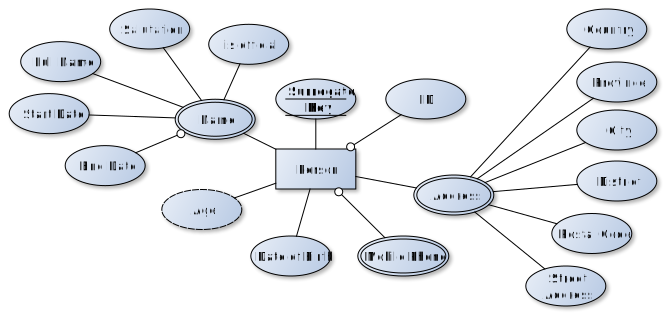
\includegraphics[width=0.95\linewidth]{\currentDir/graphics/erdPerson1}%
\end{center}%
\qENDE{%
Explain all entity types, attributes, primary keys, relationships, as well as relationship cardinalities and \nobreakdashes-modalities (as far as defined) in the \glsShort{ERD} above.%
}{%
Erklären Sie alle Entitätstypen, Attribute, Primärschlüssel, Beziehungen, sowie Beziehungskardinalitäten und \nobreakdashes-modalitäten, soweit vorhanden, in dem \glsShort{ERD} oben.%
}%
\end{question}%
%
%
%
\begin{questionENDE}{Simple Single-Valued Attribute}{Einfaches Einwertiges Attribut}%
\qENDE{%
Explain what a simple single-valued attribute is in the entity-relationship model. %
Give an example.%
}{%
Erklären Sie, was ein einfaches einwertiges Attribute in einem Entity-Relationship-Modell ist. %
Geben Sie ein Beispiel.%
}%
\end{questionENDE}%
%
%
\begin{question}{ERDs}%
\begin{center}%
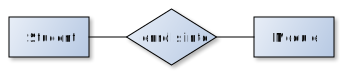
\includegraphics[width=0.5\linewidth]{\currentDir/graphics/erdStudentModule1}%
\end{center}%
\qENDE{%
Explain all entity types, attributes, primary keys, relationships, as well as relationship cardinalities and \nobreakdashes-modalities (as far as defined) in the \glsShort{ERD} above.%
}{%
Erklären Sie alle Entitätstypen, Attribute, Primärschlüssel, Beziehungen, sowie Beziehungskardinalitäten und \nobreakdashes-modalitäten, soweit vorhanden, in dem \glsShort{ERD} oben.%
}%
\end{question}%
%
\begin{questionENDE}{Office ERD}{Büros ERD}%
\qENDE{%
Design an Entity-Relationship Model~(using the original notation with rectangles, diamonds, and ellipses) for this scenario: %
Every office has a room number. %
Every employee has a name, title, and worker's number. %
Every office offers some work stations, each of which having a station number. %
Every employee occupies one of the work stations, starting from a certain date. %
Every office has one or multiple telephones, each with a certain phone number.%
}{%
Entwerfen Sie ein Entity-Relationship Modell~(in der Originalnotation mit Rechtecken, Rauten und Ellipsen) für folgende Situation: %
Jedes Büro hat eine Zimmernummer. %
Jeder Mitarbeiter hat einen Name, Titel und Arbeiternummer. %
Jedes Büro bietet eine Menge von Arbeitsplätzen, die jeweils eine Platznummer haben. %
Jeder Mitarbeiter sitzt ab einem gewissen Datum an einem der Arbeitsplätze. %
In jedem Büro gibt es ein or mehrere Telefone mit jeweils einer festen Telefonnummer.%
}%
\end{questionENDE}%
%
%
\begin{questionENDE}{Bad Practices}{Schleche Praxis}%
\qENDE{%
Why is it often a bad idea to model addresses as single text strings? %
Give one idea on how to model them better.%
}{%
Warum ist es oft eine schlechte Idee, Adressen als einfache Zeichenketten zu modellieren? %
Machen Sie einen Vorschlag, wie man sie besser modellieren kann.%
}%
\end{questionENDE}%
%
\begin{questionENDE}{Relationship Cardinality and Modality}{Beziehungskardinalität und -modalität}%
\qENDE{%
Express the following relationship with Crow's Foot notation:~\inQuotes{%
Every bank account belongs to exactly one person. %
Each person in the bank database has at least one bank account.%
}%
}{%
Drücken Sie die folgende Beziehung mit der Krähenfußnotation aus:~\inQuotes{%
Jedes Bankkonto gehört zu genau einer Person. %
Jede Person in der Bank-Datenbank hat mindestens ein Bankkonto.%
}%
}%
\end{questionENDE}%
%
%
\begin{question}{ERDs}%
\begin{center}%
\includegraphics[width=0.95\linewidth]{\currentDir/graphics/erdStudent3}%
\end{center}%
\qENDE{%
Explain all entity types, attributes, primary keys, relationships, as well as relationship cardinalities and \nobreakdashes-modalities (as far as defined) in the \glsShort{ERD} above.%
}{%
Erklären Sie alle Entitätstypen, Attribute, Primärschlüssel, Beziehungen, sowie Beziehungskardinalitäten und \nobreakdashes-modalitäten, soweit vorhanden, in dem \glsShort{ERD} oben.%
}%
\end{question}%
%
\begin{questionENDE}{Relationship Cardinality and Modality}{Beziehungskardinalität und -modalität}%
\qENDE{%
Explain the meaning of the \crowsFoot{A}{O1}{B}{O1} relationship pattern. %
Give one example.%
}{%
Erklären Sie die Bedeutung des Beziehungsformats \crowsFoot{A}{O1}{B}{O1}. %
Geben Sie ein Beispiel.%
}%
\end{questionENDE}%
%
%
\begin{questionENDE}{Relationship Cardinality and Modality}{Beziehungskardinalität und -modalität}%
\qENDE{%
Explain the meaning of the \crowsFoot{S}{MM}{T}{MM} relationship pattern. %
Give one example.%
}{%
Erklären Sie die Bedeutung des Beziehungsformats \crowsFoot{S}{MM}{T}{MM}. %
Geben Sie ein Beispiel.%
}%
\end{questionENDE}%
%
\begin{question}{ERDs}%
\begin{center}%
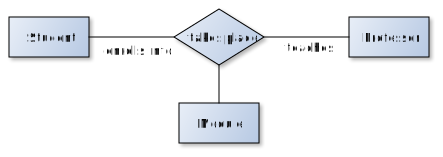
\includegraphics[width=0.5\linewidth]{\currentDir/graphics/erdStudentModuleProf2}%
\end{center}%
\qENDE{%
Explain all entity types, attributes, primary keys, relationships, as well as relationship cardinalities and \nobreakdashes-modalities (as far as defined) in the \glsShort{ERD} above.%
}{%
Erklären Sie alle Entitätstypen, Attribute, Primärschlüssel, Beziehungen, sowie Beziehungskardinalitäten und \nobreakdashes-modalitäten, soweit vorhanden, in dem \glsShort{ERD} oben.%
}%
\end{question}%
%
%
\begin{questionENDE}{Relationship Cardinality and Modality}{Beziehungskardinalität und -modalität}%
\qENDE{%
Explain the meaning of the \crowsFoot{M}{M1}{N}{MM} relationship pattern. %
Give one example.%
}{%
Erklären Sie die Bedeutung des Beziehungsformats \crowsFoot{M}{M1}{N}{MM}. %
Geben Sie ein Beispiel.%
}%
\end{questionENDE}%
%
%
\begin{questionENDE}{Relationship Cardinality and Modality}{Beziehungskardinalität und -modalität}%
\qENDE{%
Explain the meaning of the \crowsFoot{O}{OM}{P}{OM} relationship pattern. %
Give one example.%
}{%
Erklären Sie die Bedeutung des Beziehungsformats \crowsFoot{O}{OM}{P}{OM}. %
Geben Sie ein Beispiel.%
}%
\end{questionENDE}%
%
%
%
\begin{questionENDE}{Compositie Multi-Valued Attribute}{Zusammengesetztes Mehrwertiges Attribut}%
\qENDE{%
Explain what a compositve multi-valued attribute is in the entity-relationship model. %
Give an example.%
}{%
Erklären Sie, was ein zusammengesetztes mehrwertiges Attribute in einem Entity-Relationship-Modell ist. %
Geben Sie ein Beispiel.%
}%
\end{questionENDE}%
%
\begin{question}{ERDs}%
\begin{center}%
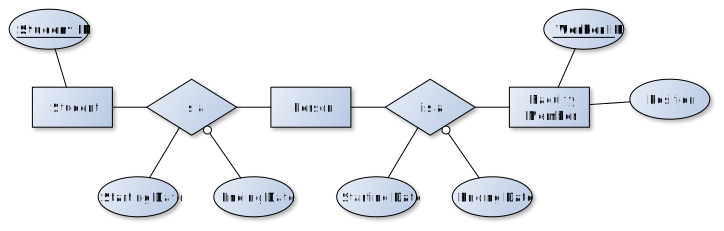
\includegraphics[width=0.95\linewidth]{\currentDir/graphics/erdPersonStudentFaculty1}%
\end{center}%
\qENDE{%
Explain all entity types, attributes, primary keys, relationships, as well as relationship cardinalities and \nobreakdashes-modalities (as far as defined) in the \glsShort{ERD} above.%
}{%
Erklären Sie alle Entitätstypen, Attribute, Primärschlüssel, Beziehungen, sowie Beziehungskardinalitäten und \nobreakdashes-modalitäten, soweit vorhanden, in dem \glsShort{ERD} oben.%
}%
\end{question}%
%
\begin{question}{ERDs}%
\begin{center}%
\includegraphics[width=0.95\linewidth]{\currentDir/graphics/erdStudent5}%
\end{center}%
\qENDE{%
Explain all entity types, attributes, primary keys, relationships, as well as relationship cardinalities and \nobreakdashes-modalities (as far as defined) in the \glsShort{ERD} above.%
}{%
Erklären Sie alle Entitätstypen, Attribute, Primärschlüssel, Beziehungen, sowie Beziehungskardinalitäten und \nobreakdashes-modalitäten, soweit vorhanden, in dem \glsShort{ERD} oben.%
}%
\end{question}%
%
\begin{questionENDE}{Relationship Cardinality and Modality}{Beziehungskardinalität und -modalität}%
\qENDE{%
Express the following relationship with Crow's Foot notation:~\inQuotes{%
A primary school student can either be subscribed to a meal plan or not. %
To a meal plan, an arbitrary number of primary school student can be subscribed.%
}%
}{%
Drücken Sie die folgende Beziehung mit der Krähenfußnotation aus:~\inQuotes{%
Ein Grundschüler kann entweder einen Essensplan aboniert haben oder nicht. %
Jeder Essensplan kann von einer beliebigen Anzahl von Grundschülern aboniert werden.%
}%
}%
\end{questionENDE}%
%
\begin{questionENDE}{Furniture ERD}{Möbel ERD}%
\qENDE{%
Design an Entity-Relationship Model~(using the original notation with rectangles, diamonds, and ellipses) for this scenario: %
A furniture store sells furniture. %
Each type of furniture has a type-ID, a name, and a price. %
It can be purchased and sold in variants, which are characterized by a name, color, and wood pattern. %
It is produced by a vendor, which is characterized by a vendor-ID, a name, and an address. %
The store has several warehouses, each of which has a name and stores amounts for different variant of different furniture types.
The company has salespeople~(employee-ID, name, date of birth, date of hiring, salary).
A salesperson can acquire and be responsible for arbitrarily many customers~(customer-ID, name, address).
The customers can issue purchase orders, characterized by an order-ID, furniture variant, amount, and deadline.%
}{%
Entwerfen Sie ein Entity-Relationship Modell~(in der Originalnotation mit Rechtecken, Rauten und Ellipsen) für folgende Situation: %
Ein Möbelladen verkauft Möbel. %
Jeder Möbel-Typ hat eine Typ-ID, einen Namen und einen Preis. %
Möbel eines Types kann in verschiedenen Varianten gekauft und verkauft werden, welche jeweils einen Namen, eine Farbe und eine Holzmaserung aufweisen. %
Ein Möbeltyp wird von einem Anbieter hergestellt, der eine Anbieter-ID, einen Namen und eine Adresse hat. %
Jede der Lagerhalle des Möbelladens hat einen Namen und kann Anzahlen verschiedener Varianten verschiedener Möbeltypen speichern. %
Der Laden hat Verkäufer~(Verkäufer-ID, Name, Geburtsdatum, Einstellungsdatum, Gehalt).
Ein Verkäufer kann beliebig viele Kunden~(Kunden-ID, Name, Adresse) anwerben und für diese verantwortlich sein. %
Ein Kunde kann Bestellungen aufgeben, die jeweils eine Bestellungs-ID, Variante eines Möbeltyps, Anzahl und Deadline haben.%
%
}%
\end{questionENDE}%
%
%
\begin{question}{ERDs}%
\begin{center}%
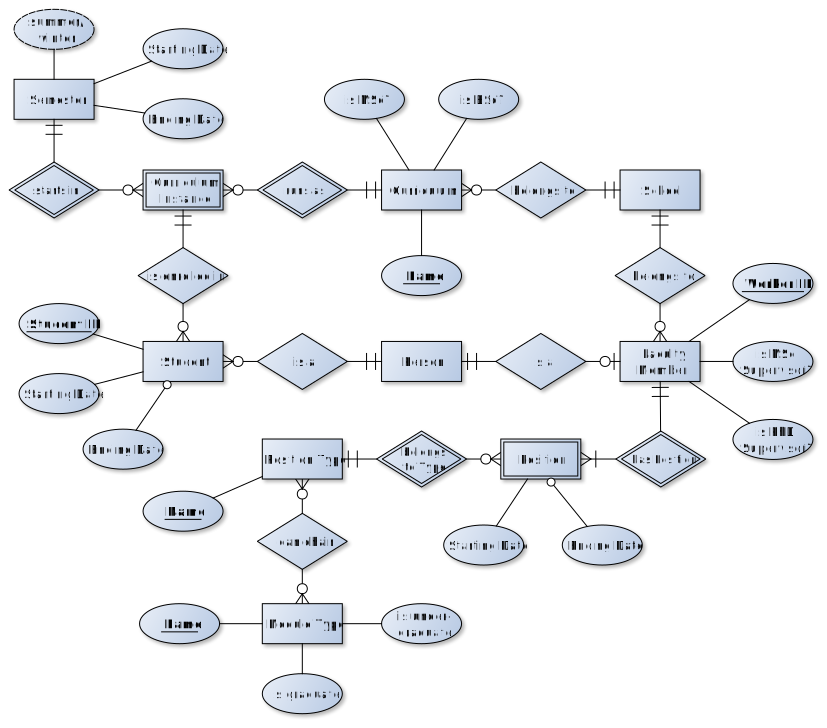
\includegraphics[width=0.95\linewidth]{\currentDir/graphics/erdPersonStudentFaculty2}%
\end{center}%
\qENDE{%
Explain all entity types, attributes, primary keys, relationships, as well as relationship cardinalities and \nobreakdashes-modalities (as far as defined) in the \glsShort{ERD} above.%
}{%
Erklären Sie alle Entitätstypen, Attribute, Primärschlüssel, Beziehungen, sowie Beziehungskardinalitäten und \nobreakdashes-modalitäten, soweit vorhanden, in dem \glsShort{ERD} oben.%
}%
\end{question}%
%
%
\begin{questionENDE}{Bad Practices}{Schleche Praxis}%
\qENDE{%
Explain an example szenario where using the telephone number as a primary key for identifying people in a database can be a problem.%
}{%
Geben Sie ein Beispielszenario an, wo das Verwenden der Telefonnummer als Primärschlüssel um Personen zu identifizieren problematisch werden kann.%
}%
\end{questionENDE}%
%
%
%
\begin{questionENDE}{Weak Entities}{Schwache Entitäten}%
\qENDE{%
Explain what a weak entity is in the entity-relationship model. %
Why do we need weak entities? %
Give an example.%
}{%
Erklären Sie, was eine schwache Entität in einem Entity-Relationship-Modell ist. %
Wofür brauchen wir schwachte Entitäten? %
Geben Sie ein Beispiel.%
}%
\end{questionENDE}%
%
\begin{questionENDE}{Soccer ERD}{Fußball ERD}%
\qENDE{%
Design an Entity-Relationship Model~(using the original notation with rectangles, diamonds, and ellipses) for this scenario: %
We develop a soccer \db. %
Every player has a name and age.
Ever game takes place on a certain game day. %
Every team has a name and a hometown. %
In each game, one team participates as home team and one as guest team. %
We store which player plays in which game, together with the starting and ending minute of their participation. %
Every team has a trainer, of whom we store name and age.%
}{%
Entwerfen Sie ein Entity-Relationship Modell~(in der Originalnotation mit Rechtecken, Rauten und Ellipsen) für folgende Situation: %
Es wird eine Fußballdatenbank entwickelt. %
Jeder Spieler hat einen Namen und ein Alter. %
Jedes Spiel findet an einem Spieltag statt. %
Jede Mannschaft hat einen Namen und einen Heimatort. %
An jedem Spiel nimmt eine Mannschaft als Heimteam und eine Mannschaft als Gast teil. %
Es wird gespeichert, an welchem Spiel welcher Spieler teilgenommen hat und zwar jeweils die Anfangs- und die Ende-Minute seines Einsatzes. %
Jede Mannschaft hat einen Trainer, dessen Name und Alter gespeichert werden.%
}%
\end{questionENDE}%
%
\begin{question}{ERDs}%
\begin{center}%
\includegraphics[width=0.8\linewidth]{\currentDir/graphics/erdStudentModuleProf1}%
\end{center}%
\qENDE{%
Explain all entity types, attributes, primary keys, relationships, as well as relationship cardinalities and \nobreakdashes-modalities (as far as defined) in the \glsShort{ERD} above.%
}{%
Erklären Sie alle Entitätstypen, Attribute, Primärschlüssel, Beziehungen, sowie Beziehungskardinalitäten und \nobreakdashes-modalitäten, soweit vorhanden, in dem \glsShort{ERD} oben.%
}%
\end{question}%
%
%
%
\begin{question}{ERDs}%
\begin{center}%
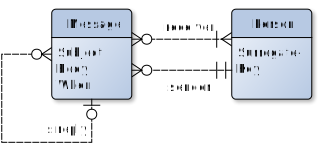
\includegraphics[width=0.5\linewidth]{\currentDir/graphics/erdMessage1}%
\end{center}%
\qENDE{%
Explain all entity types, attributes, primary keys, relationships, as well as relationship cardinalities and \nobreakdashes-modalities (as far as defined) in the \glsShort{ERD} above.%
}{%
Erklären Sie alle Entitätstypen, Attribute, Primärschlüssel, Beziehungen, sowie Beziehungskardinalitäten und \nobreakdashes-modalitäten, soweit vorhanden, in dem \glsShort{ERD} oben.%
}%
\end{question}%
%
\begin{question}{ERDs}%
\begin{center}%
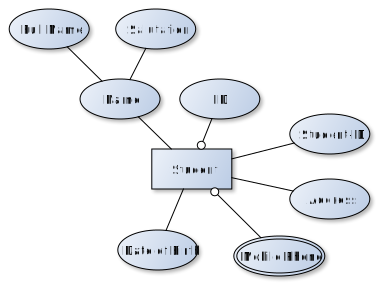
\includegraphics[width=0.5\linewidth]{\currentDir/graphics/erdStudent2}%
\end{center}%
\qENDE{%
Explain all entity types, attributes, primary keys, relationships, as well as relationship cardinalities and \nobreakdashes-modalities (as far as defined) in the \glsShort{ERD} above.%
}{%
Erklären Sie alle Entitätstypen, Attribute, Primärschlüssel, Beziehungen, sowie Beziehungskardinalitäten und \nobreakdashes-modalitäten, soweit vorhanden, in dem \glsShort{ERD} oben.%
}%
\end{question}%
%
%
\begin{questionENDE}{Relationship Cardinality and Modality}{Beziehungskardinalität und -modalität}%
\qENDE{%
Explain the meaning of the \crowsFoot{C}{O1}{D}{M1} relationship pattern. %
Give one example.%
}{%
Erklären Sie die Bedeutung des Beziehungsformats \crowsFoot{C}{O1}{D}{M1}. %
Geben Sie ein Beispiel.%
}%
\end{questionENDE}%
%
\begin{questionENDE}{Airline ERD}{Fluggesellschaft ERD}%
\qENDE{%
Design an Entity-Relationship Model~(using the original notation with rectangles, diamonds, and ellipses) for this scenario: %
Every airline has a name, home country, hometown, and abbreviation. %
An airplane has an airplane number and date of last inspection. %
Each airplane belongs to a given type, which is described by its name, number of seats, and top speed. %
Each airplane also belongs to a given airline since a certain date. %
Each pilot has a name, pilot number, qualification level, and flight hours. %
Each pilot works for a given airline since a specific date. %
Passengers are characterized by a passenger number, name, data of birth, and address.
Flights have flight number, date, start airport, destination airport, and flight time.
Each passenger can book an arbitrary number of such flights. %
A flight is realized by a given pilot and airplane.%
}{%
Entwerfen Sie ein Entity-Relationship Modell~(in der Originalnotation mit Rechtecken, Rauten und Ellipsen) für folgende Situation: %
Jede Fluggesellschaft hat einen Namen, ein Heimatland, eine Heimatstadt und eine Abkürzung. %
Jedes Flugzeug hat eine Flugzeugnummer und ein Datum der letzten Inspektion. %
Jedes Flugzeug hat einen bestimmten Typ, der durch seinen Name, die Anzahl der Sitzplätze und die Höchstgeschwindikeit charakterisiert wird. %
Jedes Flugzeug gehört zu einer Fluggesellschaft ab einem bestimmten Datum. %
Jeder Pilot hat einen Namen, eine Pilotennummer, eine Qualifikation und eine Anzahl von Flugstunden. %
Jeder Pilot arbeitet für eine bestimmte Fluggesellschaft ab einem bestimmten Datum. %
Passagiere werden charakterisiert durch eine Passagiernummer, Name, Geburtsdatum und Adresse. %
Flüge haben Flugnummern, Datum, Startflughafen, Zielflughafen und eine Flugzeit. %
Jeder Passagier kann eine beliebge Anzahl Flüge buchen. %
Ein Flug wird von einem bestimmten Pilot und Flugzeug realisiert.%
}%
\end{questionENDE}%
%
%
\begin{question}{ERDs}%
\begin{center}%
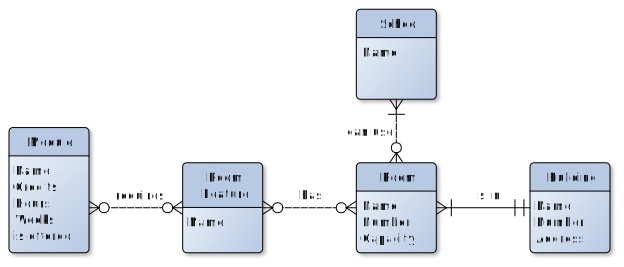
\includegraphics[width=0.8\linewidth]{\currentDir/graphics/erdRoom1}%
\end{center}%
\qENDE{%
Explain all entity types, attributes, primary keys, relationships, as well as relationship cardinalities and \nobreakdashes-modalities (as far as defined) in the \glsShort{ERD} above.%
}{%
Erklären Sie alle Entitätstypen, Attribute, Primärschlüssel, Beziehungen, sowie Beziehungskardinalitäten und \nobreakdashes-modalitäten, soweit vorhanden, in dem \glsShort{ERD} oben.%
}%
\end{question}%
%
\begin{questionENDE}{Relationship Cardinality and Modality}{Beziehungskardinalität und -modalität}%
\qENDE{%
Explain the meaning of the \crowsFoot{K}{M1}{L}{OM} relationship pattern. %
Give one example.%
}{%
Erklären Sie die Bedeutung des Beziehungsformats \crowsFoot{K}{M1}{L}{OM}. %
Geben Sie ein Beispiel.%
}%
\end{questionENDE}%
%
\begin{question}{ERDs}%
\begin{center}%
\includegraphics[width=0.8\linewidth]{\currentDir/graphics/erdStudent4}%
\end{center}%
\qENDE{%
Explain all entity types, attributes, primary keys, relationships, as well as relationship cardinalities and \nobreakdashes-modalities (as far as defined) in the \glsShort{ERD} above.%
}{%
Erklären Sie alle Entitätstypen, Attribute, Primärschlüssel, Beziehungen, sowie Beziehungskardinalitäten und \nobreakdashes-modalitäten, soweit vorhanden, in dem \glsShort{ERD} oben.%
}%
\end{question}%
%
\begin{questionENDE}{Bad Practices}{Schleche Praxis}%
\qENDE{%
Why is it generally a bad idea to assume that names can be primary keys for identifying people? %
Give an example when this becomes problematic.%
}{%
Warum ist es prinzipiell eine schlechte Idee, Namen als Primärschlüssel zum Identifizieren von Leuten zu verwenden? %
Geben Sie ein Beispielszenario, wo das schief geht.%
}%
\end{questionENDE}%
%
\begin{questionENDE}{Relationship Cardinality and Modality}{Beziehungskardinalität und -modalität}%
\qENDE{%
Explain the meaning of the \crowsFoot{G}{O1}{H}{MM} relationship pattern. %
Give one example.%
}{%
Erklären Sie die Bedeutung des Beziehungsformats \crowsFoot{G}{O1}{H}{MM}. %
Geben Sie ein Beispiel.%
}%
\end{questionENDE}%
%
\begin{questionENDE}{Company ERD}{Firma ERD}%
\qENDE{%
Design an Entity-Relationship Model~(using the original notation with rectangles, diamonds, and ellipses) for this scenario: %
Every work group has a group number, name, and location. %
Every employee has a worker's number, name, date of birth, salary, address, and job. %
Every employee belongs to a work group. %
Each project has a name and deadline. %
Every employee works on at least one, but maybe multiple projects. %
Each project has an employee as a leader.%
}{%
Entwerfen Sie ein Entity-Relationship Modell~(in der Originalnotation mit Rechtecken, Rauten und Ellipsen) für folgende Situation: %
Jede Arbeitsgruppe hat eine Gruppennummer, Name und Ort. %
Jeder Mitarbeiter hat eine Arbeiternummer, Name, Geburtsdatum, Gehalt, Adresse und Arbeitsaufgabe. %
Jeder Mitarbeiter gehört zu einer Arbeitsgruppe. %
Jedes Projekt hat einen Namen und eine Deadline. %
Jeder Mitarbeiter arbeitet an mindestens einem, vielleicht aber auch mehreren Projekten. %
Jedes Projekt hat einen Mitarbeiter als Leiter.%
}%
\end{questionENDE}%
%
%
\begin{questionENDE}{Relationship Cardinality and Modality}{Beziehungskardinalität und -modalität}%
\qENDE{%
Explain the meaning of the \crowsFoot{E}{O1}{F}{OM} relationship pattern. %
Give one example.%
}{%
Erklären Sie die Bedeutung des Beziehungsformats \crowsFoot{E}{O1}{F}{OM}. %
Geben Sie ein Beispiel.%
}%
\end{questionENDE}%
%
\begin{question}{ERDs}%
\begin{center}%
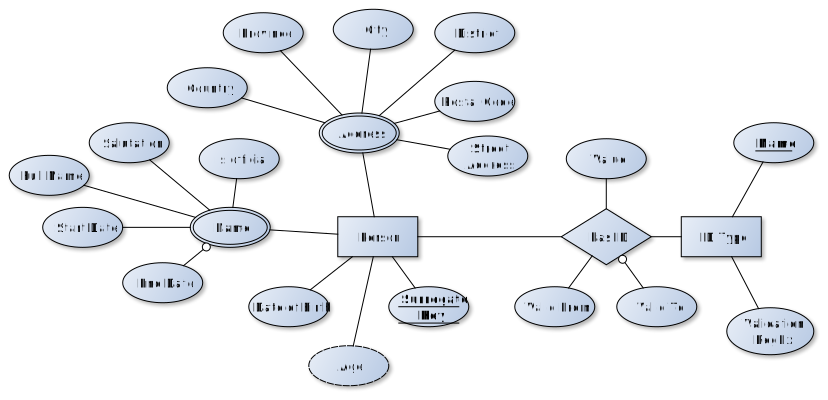
\includegraphics[width=0.95\linewidth]{\currentDir/graphics/erdPerson2}%
\end{center}%
\qENDE{%
Explain all entity types, attributes, primary keys, relationships, as well as relationship cardinalities and \nobreakdashes-modalities (as far as defined) in the \glsShort{ERD} above.%
}{%
Erklären Sie alle Entitätstypen, Attribute, Primärschlüssel, Beziehungen, sowie Beziehungskardinalitäten und \nobreakdashes-modalitäten, soweit vorhanden, in dem \glsShort{ERD} oben.%
}%
\end{question}%
%
\begin{question}{ERDs}%
\begin{center}%
\includegraphics[width=0.5\linewidth]{\currentDir/graphics/erdStudentModuleProf3}%
\end{center}%
\qENDE{%
Erklären Sie alle Entitätstypen, Attribute, Primärschlüssel, Beziehungen, sowie Beziehungskardinalitäten und \nobreakdashes-modalitäten, soweit vorhanden, in dem \glsShort{ERD} oben.%
}{%
Explain all entity types, attributes, primary keys, relationships, as well as relationship cardinalities and \nobreakdashes-modalities (as far as defined) in the \glsShort{ERD} above.%
}%
\end{question}%
%
%
\begin{questionENDE}{Relationship Cardinality and Modality}{Beziehungskardinalität und -modalität}%
\qENDE{%
Express the following relationship with Crow's Foot notation:~\inQuotes{%
Every student is enrolled into at least one lecture. %
Into each lecture, at least one student is enrolled.%
}%
}{%
Drücken Sie die folgende Beziehung mit der Krähenfußnotation aus:~\inQuotes{%
Jeder Student ist in mindestens eine Vorlesung eingeschrieben. %
In jede Vorlesung ist mindestens ein Student eingeschrieben.%
}%
}%
\end{questionENDE}%
%
%
%
\begin{questionENDE}{Simple Multi-Valued Attribute}{Einfaches Mehrwertiges Attribut}%
\qENDE{%
Explain what a simple multi-valued attribute is in the entity-relationship model. %
Give an example.%
}{%
Erklären Sie, was ein einfaches mehrwertiges Attribute in einem Entity-Relationship-Modell ist. %
Geben Sie ein Beispiel.%
}%
\end{questionENDE}%
%
%
\begin{questionENDE}{Sports ERD}{Sportarten ERD}%
\qENDE{%
Design an Entity-Relationship Model~(using the original notation with rectangles, diamonds, and ellipses) for this scenario: %
Every sports discipline has a name and a world, asia-, and olympic record. %
There are competitions which have a competition number, date, location, start time, and type. %
The competition type has a name, e.g., Asian Championship, Olympics, etc. %
Every athlete has a name, age, sports club, and home country. %
Every competition offers a set of sports disciplines and athletes can take part in multiple disciplines in multiple competitions. %
Each athlete has a trainer, for whom we store the qualification, name, and date of birth. %
A trainer can train arbitrarily many athletes.%
}{%
Entwerfen Sie ein Entity-Relationship Modell~(in der Originalnotation mit Rechtecken, Rauten und Ellipsen) für folgende Situation: %
Jede Sportdisziplin hat einen Namen und jeweils eine Welt-, Asien- und Olympiarekord. %
Es werden Wettkämpfe ausgetragen, die jeweils eine Wettkampfnummer, Datum, Ort, Uhrzeit und Art haben.
Jede Wettkampfart hat einen Namen, \DEzB\ Asienmeisterschaft, Olympiade, usw. %
Jeder Sportler hat einen Namen, Alter, Sportklub und Heimatland. %
Jeder Wettkampf kann bestimmte Sportarten anbieten und Sportler können an Wettkämpfen teilnehmen und zwar jeweils in beliebig vielen Disziplinen. %
Jeder Sportler hat einen Trainer, über den wir den Name, die Qualifikation und das Geburtsdatum speichern.%
Ein Trainer kann beliebig viele Sportler betreuen.%
}%
\end{questionENDE}%
%
%
\begin{questionENDE}{Relationship Cardinality and Modality}{Beziehungskardinalität und -modalität}%
\qENDE{%
Explain the meaning of the \crowsFoot{Q}{OM}{R}{MM} relationship pattern. %
Give one example.%
}{%
Erklären Sie die Bedeutung des Beziehungsformats \crowsFoot{Q}{OM}{R}{MM}. %
Geben Sie ein Beispiel.%
}%
\end{questionENDE}%
%
%
%
\begin{questionENDE}{Relationship Cardinality and Modality}{Beziehungskardinalität und -modalität}%
\qENDE{%
Express the following relationship with Crow's Foot notation:~\inQuotes{%
Every cook has at least one cook's hat. %
Each cook's hat belongs to exactly one cook.%
}%
}{%
Drücken Sie die folgende Beziehung mit der Krähenfußnotation aus:~\inQuotes{%
Jede Koch hat mindestens eine Kochmütze. %
Jede Kochmütze gehört genau einem Koch.%
}%
}%
\end{questionENDE}%
%
%
\begin{question}{ERDs}%
\begin{center}%
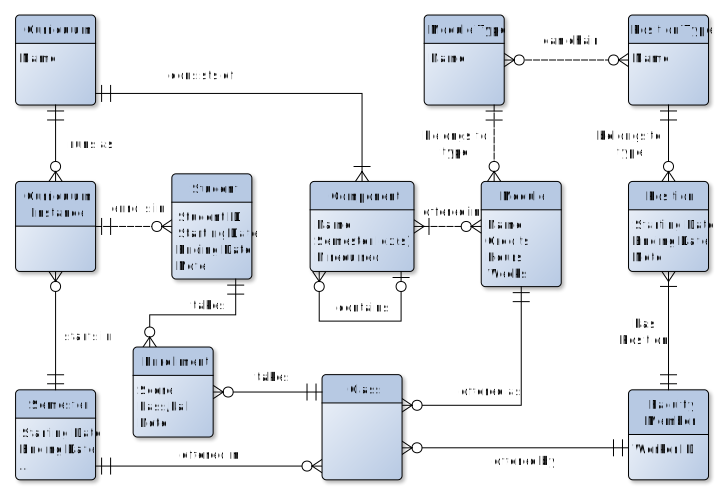
\includegraphics[width=0.9\linewidth]{\currentDir/graphics/erdModules1}%
\end{center}%
\qENDE{%
Explain all entity types, attributes, primary keys, relationships, as well as relationship cardinalities and \nobreakdashes-modalities (as far as defined) in the \glsShort{ERD} above.%
}{%
Erklären Sie alle Entitätstypen, Attribute, Primärschlüssel, Beziehungen, sowie Beziehungskardinalitäten und \nobreakdashes-modalitäten, soweit vorhanden, in dem \glsShort{ERD} oben.%
}%
\end{question}%
%
\begin{question}{ERDs}%
\begin{center}%
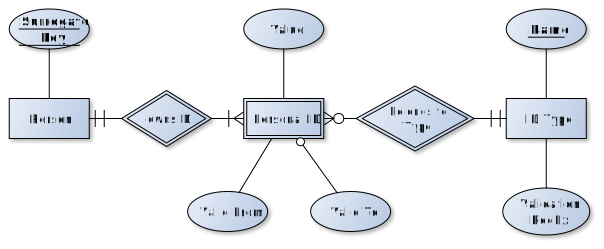
\includegraphics[width=0.8\linewidth]{\currentDir/graphics/erdPerson4}%
\end{center}%
\qENDE{%
Explain all entity types, attributes, primary keys, relationships, as well as relationship cardinalities and \nobreakdashes-modalities (as far as defined) in the \glsShort{ERD} above.%
}{%
Erklären Sie alle Entitätstypen, Attribute, Primärschlüssel, Beziehungen, sowie Beziehungskardinalitäten und \nobreakdashes-modalitäten, soweit vorhanden, in dem \glsShort{ERD} oben.%
}%
\end{question}%
%
%
\begin{questionENDE}{Relationship Cardinality and Modality}{Beziehungskardinalität und -modalität}%
\qENDE{%
Express the following relationship with Crow's Foot notation:~\inQuotes{%
Every email can either be new or the answer to an existing email. %
Each email can be answered an arbitrary number of times.%
}%
}{%
Drücken Sie die folgende Beziehung mit der Krähenfußnotation aus:~\inQuotes{%
Jede Email ist entweder neu oder ist die Antwort auf eine existierende Email. %
Jede Email kann beliebig oft beantwortet werden.%
}%
}%
\end{questionENDE}%
%
\begin{questionENDE}{Hospital ERD}{Krankenhaus ERD}%
\qENDE{%
Design an Entity-Relationship Model~(using the original notation with rectangles, diamonds, and ellipses) for this scenario: %
The work of a hospital should be stored and represented by a database. %
Each patient has a patient-ID, a name, a date of birth, an address, an entry date, and exit date, and a diagnosis. %
Each medicine has a name, a main chemical compound, and a producer. %
Each department has a name and a specialization. %
Each doctor has a doctor-ID, a name, and a phone number. %
Each doctor belongs to a department. %
Each room belongs to a department, has a room number, a number of beds, and a phone number.
Each patient belongs to a room. %
Each patient is treated by one or multiple doctors. %
Each patient gets a specific dosage (number of administrations per day, amount per administration) of one or multiple medicines.%
}{%
Entwerfen Sie ein Entity-Relationship Modell~(in der Originalnotation mit Rechtecken, Rauten und Ellipsen) für folgende Situation: %
Die Arbeit eines Krankenhauses soll in einer Datenbank repräsentiert werden. %
Jeder Patient hat eine Patienten-ID, einen Namen, ein Geburtsdatum, eine Adresse, ein Einlieferungsdatum, ein Entlassungsdatum und eine Diagnose. %
Jede Medizin hat einen Namen, einen Hauptwirkstoff und einen Produzenten. %
Jede Abteilung hat einen Namen und eine Spezialisierung. %
Jeder Arzt hat eine Arzt-ID, einen Namen und eine Telefonnummer. %
Jeder Arzt gehört zu einer Abteilung. %
Jeder Raum gehört zu einer Abteilung und hat eine Raumnummer, eine Anzahl von Betten und eine Telefonnummer. %
Jeder Patient gehört zu einem Raum. %
Jeder Patient kann von einem oder mehreren Ärzten behandelt werden. %
Jeder Patient bekommt eine bestimmte Dosierung~(Anzahl der Anwendungen pro Tag, Menge pro Anwendung) von einer oder mehrerer Medizinen.%
}%
\end{questionENDE}%
%
%
\begin{questionENDE}{Relationship Cardinality and Modality}{Beziehungskardinalität und -modalität}%
\qENDE{%
Express the following relationship with Crow's Foot notation:~\inQuotes{%
A trainer trains at least one tennis player. %
Each tennis player either has one trainer or no trainer.%
}%
}{%
Drücken Sie die folgende Beziehung mit der Krähenfußnotation aus:~\inQuotes{%
Jeder Trainer trainiert mindestens einen Tennisspieler. %
Jeder Tennisspieler hat mindestens einen Trainer.%
}%
}%
\end{questionENDE}%
%
%
%
\begin{questionENDE}{Relationship Cardinality and Modality}{Beziehungskardinalität und -modalität}%
\qENDE{%
Express the following relationship with Crow's Foot notation:~\inQuotes{%
Each vehicle has at least one wheel. %
A wheel is attached to exactly one vehicle~(or stored somewhere).%
}%
}{%
Drücken Sie die folgende Beziehung mit der Krähenfußnotation aus:~\inQuotes{%
Jedes Fahrzeug hat mindestens ein Rad. %
Jedes Rad ist mit genau einem Fahrzeug verbunden~(oder wird irgendwo gelagert.)%
}%
}%
\end{questionENDE}%
%
%
\begin{questionENDE}{Relationship Cardinality and Modality}{Beziehungskardinalität und -modalität}%
\qENDE{%
Explain the meaning of the \crowsFoot{I}{M1}{J}{M1} relationship pattern. %
Give one example.%
}{%
Erklären Sie die Bedeutung des Beziehungsformats \crowsFoot{I}{M1}{J}{M1}. %
Geben Sie ein Beispiel.%
}%
\end{questionENDE}%
%
\begin{question}{ERDs}%
\begin{center}%
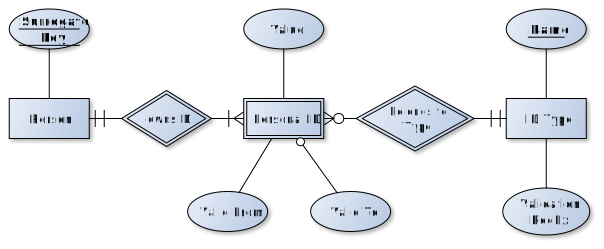
\includegraphics[width=0.85\linewidth]{\currentDir/graphics/erdPerson4}%
\end{center}%
\qENDE{%
Explain all entity types, attributes, primary keys, relationships, as well as relationship cardinalities and \nobreakdashes-modalities (as far as defined) in the \glsShort{ERD} above.%
}{%
Erklären Sie alle Entitätstypen, Attribute, Primärschlüssel, Beziehungen, sowie Beziehungskardinalitäten und \nobreakdashes-modalitäten, soweit vorhanden, in dem \glsShort{ERD} oben.%
}%
\end{question}%
%
%
\begin{questionENDE}{Compositie Single-Valued Attribute}{Zusammengesetztes Einwertiges Attribut}%
\qENDE{%
Explain what a compositve single-valued attribute is in the entity-relationship model. %
Give an example.%
}{%
Erklären Sie, was ein zusammengesetztes einwertiges Attribute in einem Entity-Relationship-Modell ist. %
Geben Sie ein Beispiel.%
}%
\end{questionENDE}%
%
%
\begin{question}{ERDs}%
\begin{center}%
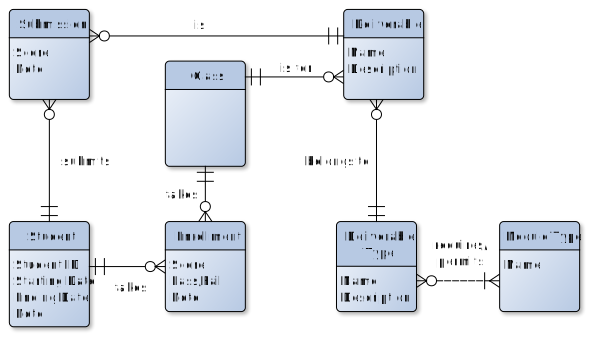
\includegraphics[width=0.8\linewidth]{\currentDir/graphics/erdDeliverables1}%
\end{center}%
\qENDE{%
Explain all entity types, attributes, primary keys, relationships, as well as relationship cardinalities and \nobreakdashes-modalities (as far as defined) in the \glsShort{ERD} above.%
}{%
Erklären Sie alle Entitätstypen, Attribute, Primärschlüssel, Beziehungen, sowie Beziehungskardinalitäten und \nobreakdashes-modalitäten, soweit vorhanden, in dem \glsShort{ERD} oben.%
}%
\end{question}%
%
\begin{question}{ERDs}%
\begin{center}%
\includegraphics[width=0.8\linewidth]{\currentDir/graphics/erdPerson3}%
\end{center}%
\qENDE{%
Explain all entity types, attributes, primary keys, relationships, as well as relationship cardinalities and \nobreakdashes-modalities (as far as defined) in the \glsShort{ERD} above.%
}{%
Erklären Sie alle Entitätstypen, Attribute, Primärschlüssel, Beziehungen, sowie Beziehungskardinalitäten und \nobreakdashes-modalitäten, soweit vorhanden, in dem \glsShort{ERD} oben.%
}%
\end{question}%
%
\begin{question}{ERDs}%
\begin{center}%
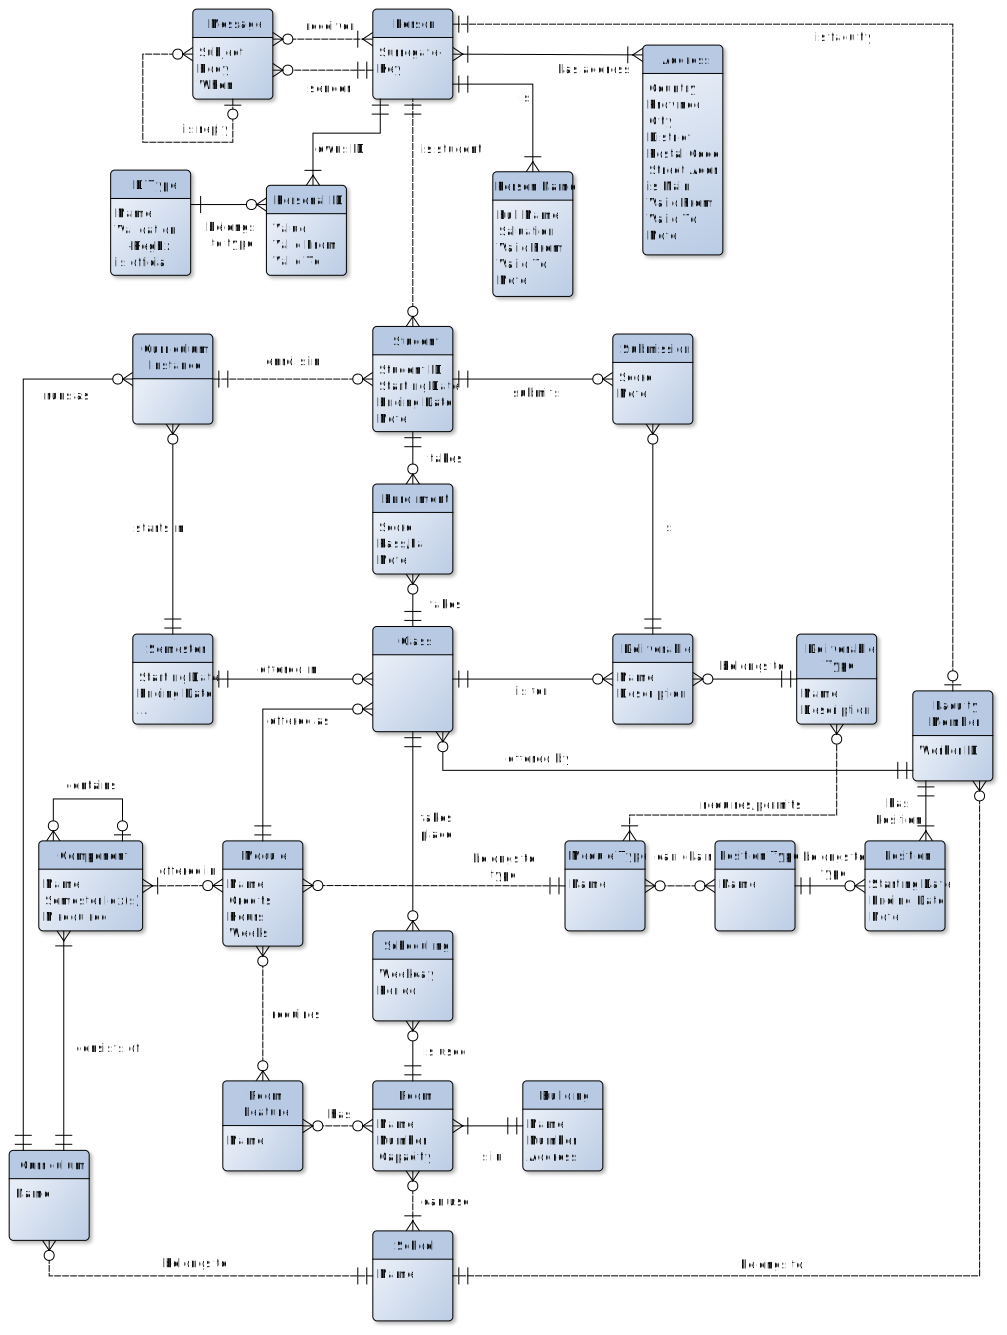
\includegraphics[width=0.95\linewidth]{\currentDir/graphics/erdPlatform1}%
\end{center}%
\qENDE{%
Explain all entity types, attributes, primary keys, relationships, as well as relationship cardinalities and \nobreakdashes-modalities (as far as defined) in the \glsShort{ERD} above.%
}{%
Erklären Sie alle Entitätstypen, Attribute, Primärschlüssel, Beziehungen, sowie Beziehungskardinalitäten und \nobreakdashes-modalitäten, soweit vorhanden, in dem \glsShort{ERD} oben.%
}%
\end{question}%
%
%
\begin{questionENDE}{Weak and Strong Entities}{Schwache und Starke Entitäten}%
\qENDE{%
Explain what weak and strong entities are in the entity-relationship model. %
What is their difference? %
Why do we need weak entities?
Give an example for each.%
}{%
Erklären Sie, was schwache und starke Entitäten in einem Entity-Relationship-Modell sind. %
Was ist der Unterschied zwischen beiden? %
Wofür brauchen wir schwachte Entitäten? %
Geben Sie jeweils ein Beispiel.%
}%
\end{questionENDE}%
%
%
\begin{questionENDE}{Relationship Cardinality and Modality}{Beziehungskardinalität und -modalität}%
\qENDE{%
Explain the meaning of the \crowsFoot{A}{O1}{B}{O1} relationship pattern. %
Give one example.%
}{%
Erklären Sie die Bedeutung des Beziehungsformats \crowsFoot{A}{O1}{B}{O1}. %
Geben Sie ein Beispiel.%
}%
\end{questionENDE}%
%
\endhsection%
